% !TeX root=main.tex
\chapter{معماری سیستم بلاکچین پیشنهادی}
%\thispagestyle{empty} 

\section{مقدمه}
در این فصل به تشریح معماری سیستم بلاکچین پیشنهادی می‌پردازیم. معماری پیشنهادی از ساختار زنجیره اصلی \lr{(Master Chain)} و مجموعه‌ای از زنجیره‌های جانبی \lr{(Side Chains)} استفاده می‌کند. برخلاف بسیاری از راه‌حل‌های \lr{L2} که تراکنش را به‌طور کامل خارج از زنجیره نگه می‌دارند، این طرح \textbf{پردازش موازی روی زنجیره‌های مستقل} را با \textbf{ثبت دوره‌ای ارجاع در زنجیره اصلی} ترکیب می‌کند.

ابتدا مسئله و شاخص‌ها را در قالب مدل سیستم (مشابه الگوریتم‌های اجماع) تعریف می‌کنیم، سپس معماری، الگوریتم‌ها و مقایسه مقیاس‌پذیری با روش‌های مشابه را ارائه می‌دهیم. نتایج عددی بنچمارک در فصل چهارم گزارش می‌شود.

\section{مدل رسمی مسئله و شاخص‌ها}

\subsection{مدل سیستم}

\begin{definition}[سیستم چندزنجیره‌ای]
یک سیستم چندزنجیره‌ای را با هفت‌تایی زیر در نظر می‌گیریم:
\begin{latin}
\[
\mathcal{S} = \langle \mathcal{P},\ C_0,\ \{C_i\}_{i=1}^{N},\ \mathcal{U},\ \mathcal{M},\ \mathcal{A} \rangle
\]
\end{latin}
که در آن $\mathcal{P}$ مجموعه فرآیندها (نودها/ماینرها)، $C_0$ زنجیره اصلی، $C_i$ زنجیره جانبی $i$ام، $\mathcal{U}$ مجموعه \lr{UTXO}های معتبر، $\mathcal{M}$ مجموعه \lr{mempool}ها (یک \lr{mempool} به ازای هر $C_i$) و $\mathcal{A}$ تابع تخصیص قطعی است.
\end{definition}

هر بلوک زنجیره اصلی هر $\Delta T_m$ ثانیه (مثلاً ۶۰۰) تولید می‌شود و مجموعه‌ای از \textbf{ارجاعات} به هدر بلوک‌های زنجیره‌های جانبی را در خود دارد. هر بلوک زنجیره جانبی هر $\Delta T_s$ ثانیه (مثلاً ۶۰) تولید می‌شود و مجموعه‌ای از تراکنش‌ها را در بر می‌گیرد.

\subsection{تخصیص قطعی}

\begin{definition}[تابع تخصیص]
برای $N$ زنجیره جانبی، تخصیص هر \lr{UTXO} به شناسه زنجیره:
\begin{latin}
\[
\mathcal{A}(\mathit{utxo}) = H(\mathit{utxo}) \bmod N
\]
\end{latin}
که $H$ تابع هش رمزنگاری (\lr{SHA-256}) و خروجی به بازه $\{0,\ldots,N-1\}$ نگاشت می‌شود.
\end{definition}

\subsection{خواص صحت (Validity, Agreement, Termination)}

الگوریتم‌های اجماع کلاسیک سه خواص \lr{Validity}، \lr{Agreement} و \lr{Termination} را مطرح می‌کنند. در معماری پیشنهادی، خواص زیر معادل نقش مشابهی دارند:

\begin{definition}[صحت \lr{(Validity)}]
\textbf{صحت تخصیص:} هر تراکنش $tx$ تنها در زنجیره $C_{\mathcal{A}(u)}$ پذیرفته می‌شود که $u$ یک \lr{UTXO} ورودی معتبر $tx$ باشد و $tx$ از نظر امضا، مبلغ و عدم دوبارخرج معتبر باشد.

\textbf{صحت ارجاع:} هر ارجاع $r$ در بلوک $C_0$ به هدر بلوکی اشاره می‌کند که واقعاً در $C_i$ استخراج شده و هش آن با $r$ سازگار است.
\end{definition}

\begin{definition}[توافق \lr{(Agreement)}]
تمام نودهای صادق بر (۱) مقدار $\mathcal{A}(u)$ برای هر \lr{UTXO}، (۲) ترتیب بلوک‌های $C_0$ بر اساس بیشترین کار انجام‌شده \lr{(PoW)}، و (۳) مجموعه ارجاعات ثبت‌شده در هر بلوک $C_0$ توافق دارند.
\end{definition}

\begin{definition}[پایان‌پذیری \lr{(Termination)}]
برای هر تراکنش معتبر $tx$ که در \lr{mempool} مربوطه قرار گیرد، پس از زمان محدود $T_{fin}$، $tx$ در یک بلوک $C_i$ گنجانده شده و هدر آن بلوک در یک بلوک $C_0$ ارجاع می‌شود؛ یعنی $tx$ \textbf{نهایی} (\lr{finalized}) می‌شود.
\end{definition}

\begin{remark}
$T_{fin}$ تقریباً برابر $k \cdot \Delta T_m$ است که $k$ عمق تأیید زنجیره اصلی (مثلاً $k=6$ مشابه بیتکوین) و $\Delta T_m$ فاصله بلوک اصلی است. زنجیره‌های جانبی تأیید اولیه سریع‌تر ($\Delta T_s$) ارائه می‌دهند؛ قطعیت امنیتی از لنگر $C_0$ حاصل می‌شود.
\end{remark}

\subsection{شاخص‌های عملکرد}

\begin{definition}[شاخص‌های مقیاس‌پذیری]
\begin{latin}
\[
TPS_{total} = \frac{M}{\Delta T_m} + \sum_{i=1}^{N}\frac{S_i}{\Delta T_s}
\approx \frac{M}{\Delta T_m} + \frac{N \cdot S}{\Delta T_s}
\]
\end{latin}
برای $M$ تراکنش (یا ارجاع) در هر بلوک اصلی، $S$ تراکنش میانگین در هر بلوک جانبی، و فرض تقارن $S_i=S$. \textbf{تأخیر اولیه} $L_0 \approx \Delta T_s$ و \textbf{تأخیر نهایی} $L_{fin} \approx k\cdot\Delta T_m$.
\end{definition}

\section{معماری کلی سیستم}

معماری پیشنهادی شامل دو لایه اصلی است. زنجیره اصلی \lr{(Master Chain)} ستون فقرات شبکه است که از الگوریتم اثبات کار \lr{(Proof of Work)} مشابه بیتکوین استفاده می‌کند. هر ۱۰ دقیقه یک بلوک جدید در زنجیره اصلی تولید می‌شود و محتوای آن شامل ارجاعات به بلوک‌های زنجیره‌های جانبی است. امنیت با استفاده از الگوریتم \lr{SHA-256} تضمین می‌شود و سطح دشواری استخراج قابل تنظیم است (معمولاً سطح بالا برای امنیت بیشتر).

ساختار یک بلوک در زنجیره اصلی به صورت زیر است:

\begin{latin}
\begin{equation}
\begin{split}
\text{MasterBlock} = \bigl\{ &\text{index},\ \text{timestamp},\ \text{references},\ \text{previous\_hash}, \\
&\text{hash},\ \text{nonce},\ \text{difficulty} \bigr\}
\end{split}
\end{equation}
\end{latin}

که در آن $index$ شماره بلوک، $timestamp$ زمان تولید، $references$ لیست ارجاعات به بلوک‌های زنجیره‌های جانبی، $previous\_hash$ و $hash$ به ترتیب هش بلوک قبلی و فعلی، $nonce$ عدد استفاده شده در استخراج و $difficulty$ سطح دشواری استخراج است.

زنجیره‌های جانبی \lr{(Side Chains)} واحدهای پردازش موازی هستند که تراکنش‌ها را به صورت مستقل پردازش می‌کنند. تعداد آن‌ها قابل تنظیم و افزایش است (مقیاس‌پذیری افقی)، هر ۱ دقیقه یک بلوک جدید تولید می‌شود و محتوای بلوک‌ها شامل تراکنش‌های واقعی کاربران است. دشواری استخراج در زنجیره‌های جانبی پایین‌تر از زنجیره اصلی است و هر بلوک زنجیره جانبی به یک بلوک در زنجیره اصلی مرتبط می‌شود.

ساختار یک بلوک در زنجیره جانبی:

\begin{latin}
\begin{equation}
\begin{split}
\text{SideChainBlock} = \bigl\{ &\text{index},\ \text{side\_chain\_id},\ \text{timestamp},\ \text{transactions}, \\
&\text{previous\_hash},\ \text{parent\_master\_hash},\ \text{hash},\ \text{nonce} \bigr\}
\end{split}
\end{equation}
\end{latin}

\begin{figure}[h]
\centering
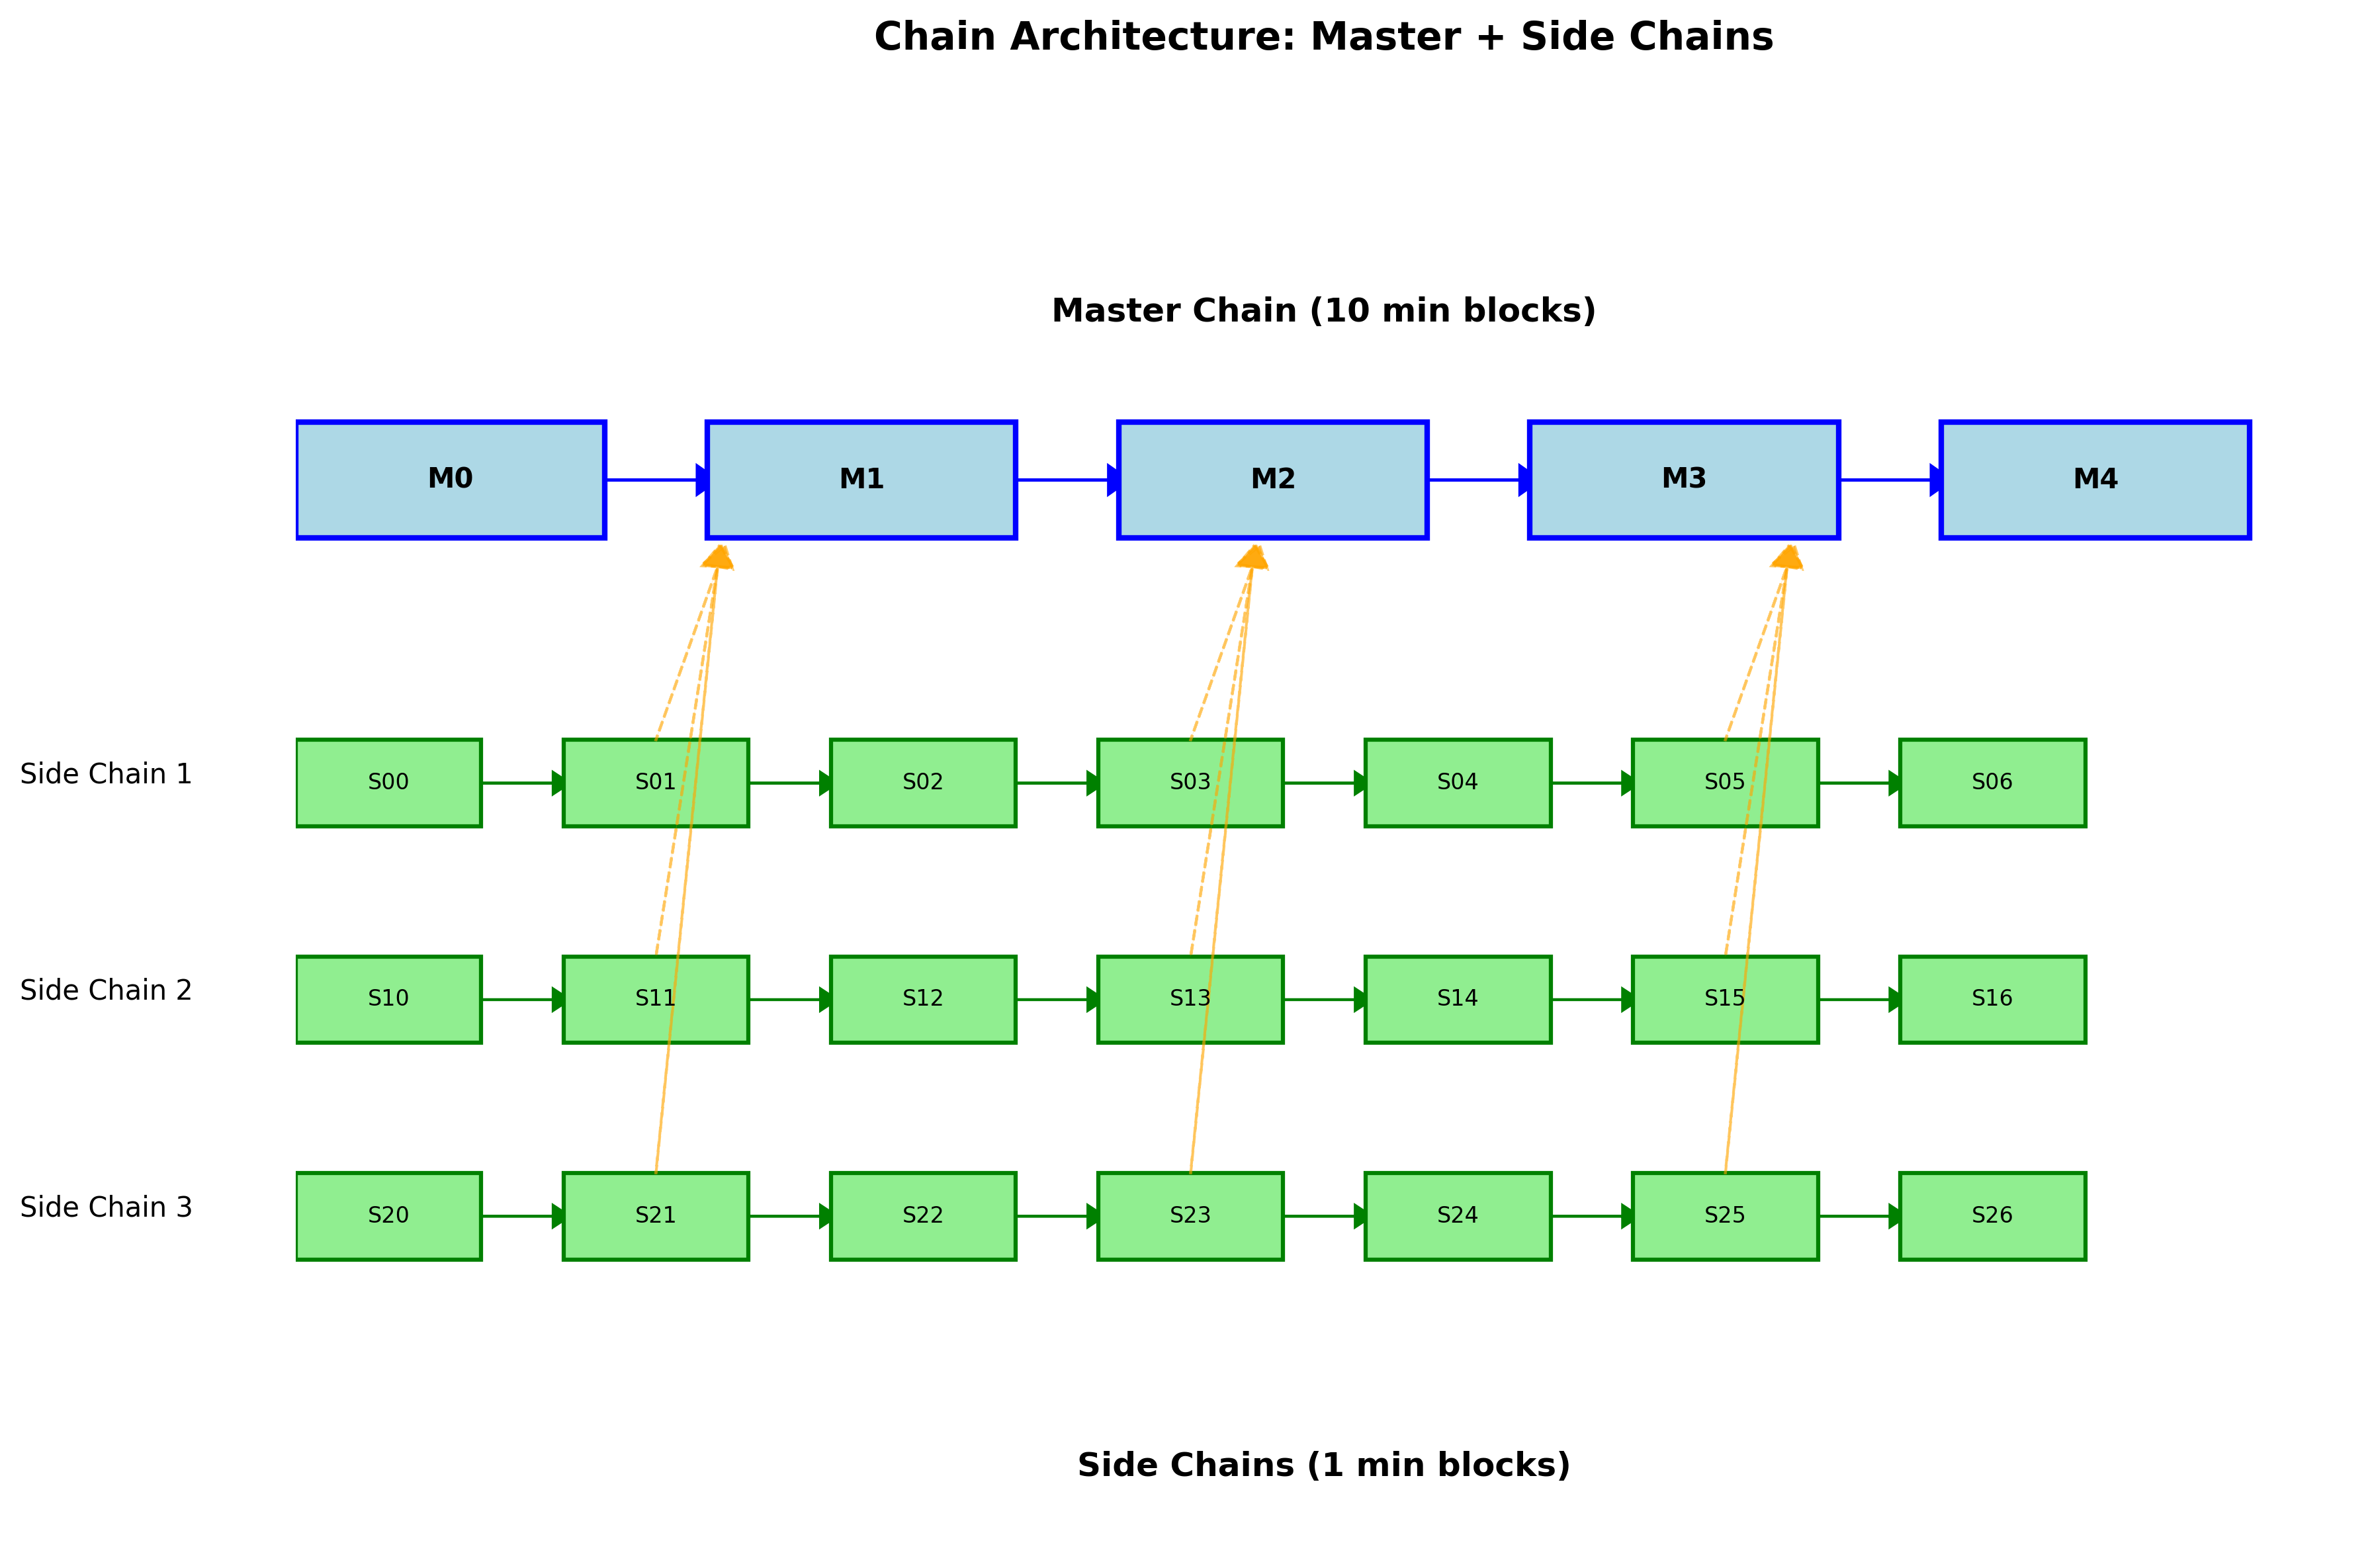
\includegraphics[width=0.9\textwidth]{img/architecture_diagram.png}
\caption{نمای کلی معماری زنجیره اصلی و زنجیره‌های جانبی}
\label{fig:architecture}
\end{figure}

\section{الگوریتم‌های کلیدی}

\subsection{الگوریتم تخصیص تراکنش}

الگوریتم \ref{alg:assign} تخصیص قطعی را پیاده می‌کند و خواص \lr{Validity} و \lr{Agreement} تخصیص را تضمین می‌کند.

\begin{algorithm}[h]
\caption{تخصیص تراکنش به زنجیره جانبی}
\label{alg:assign}
\begin{algorithmic}[1]
\REQUIRE تراکنش $tx$، تعداد زنجیره‌ها $N$
\ENSURE شناسه زنجیره $sid \in \{0,\ldots,N-1\}$
\STATE $u \gets$ اولین \lr{UTXO} ورودی $tx$
\STATE $h \gets \text{SHA256}(u)$ \COMMENT{هش ۲۵۶ بیتی}
\STATE $v \gets$ تبدیل ۸ بایت اول $h$ به عدد صحیح بی‌علامت ۶۴ بیتی
\STATE $sid \gets v \bmod N$
\RETURN $sid$
\end{algorithmic}
\end{algorithm}

پیچیدگی زمانی $O(1)$ است. در پیاده‌سازی Rust: \lr{\texttt{utxo.numeric\_hash() \% num\_side\_chains}}.

\begin{algorithm}[h]
\caption{پردازش و نهایی‌سازی تراکنش}
\label{alg:process}
\begin{algorithmic}[1]
\REQUIRE $tx$، سیستم $\mathcal{S}$
\STATE $sid \gets$ خروجی الگوریتم \ref{alg:assign}
\STATE افزودن $tx$ به $\mathcal{M}_{sid}$
\STATE استخراج بلوک $B_s$ روی $C_{sid}$ (هر $\Delta T_s$)
\STATE ساخت بلوک $B_m$ روی $C_0$ حاوی $\text{Ref}(B_s)$
\IF{$B_m$ دارای $k$ تأیید روی $C_0$}
   \STATE علامت‌گذاری $tx$ به‌عنوان \lr{finalized}
\ENDIF
\end{algorithmic}
\end{algorithm}

\subsection{اجماع و ماژول‌های پیاده‌سازی}

پیاده‌سازی Rust شامل چهار ماژول است: \textbf{رمزنگاری} (\lr{SHA-256}، \lr{ECDSA})، \textbf{اجماع} (انتخاب زنجیره با بیشترین کار، قطعیت پس از $k=6$ تأیید)، \textbf{اعتبارسنجی} (\lr{UTXO set}، جلوگیری از دوبارخرج) و \textbf{تراکنش بین‌زنجیره‌ای} (قفل اتمیک: \lr{Initiated $\rightarrow$ Locked $\rightarrow$ Verified $\rightarrow$ Completed}).

\section{فرآیند پردازش تراکنش}

فرآیند پردازش یک تراکنش مطابق الگوریتم \ref{alg:process} است: ایجاد $tx$ $\rightarrow$ تخصیص به $C_{\mathcal{A}(u)}$ $\rightarrow$ قرارگیری در \lr{mempool} $\rightarrow$ استخراج $B_s$ $\rightarrow$ ارجاع در $B_m$ $\rightarrow$ نهایی‌سازی پس از $k$ تأیید روی $C_0$.

\section{مقایسه مقیاس‌پذیری با روش‌های مشابه}

جدول \ref{tab:scalability-comparison-ch3} معماری پیشنهادی را از نظر \textbf{رشد خطی \lr{TPS}} با راه‌حل‌های مرورشده در فصل دوم مقایسه می‌کند.

\begin{table}[h]
\centering
\caption{مقایسه مقیاس‌پذیری: معماری پیشنهادی در برابر روش‌های مشابه}
\label{tab:scalability-comparison-ch3}
\small
\begin{tabular}{|p{2.8cm}|p{2.2cm}|p{2.4cm}|p{2.6cm}|p{2.4cm}|}
\hline
\textbf{روش} & \textbf{رشد \lr{TPS}} & \textbf{لنگر امنیتی} & \textbf{تغییر \lr{L1}} & \textbf{محدودیت اصلی} \\
\hline
بیتکوین & ثابت ($\sim$7) & خود \lr{L1} & --- & اندازه/فاصله بلوک \\
\hline
لایتنینگ & وابسته به کانال & \lr{L1} (تسویه) & \lr{L2} & نقدینگی، مسیریابی \\
\hline
شاردینگ & خطی با شارد & شارد + \lr{beacon} & زیاد & امنیت/ارتباط بین‌شاردی \\
\hline
زنجیره جانبی (\lr{RSK}) & محدود (یک جانبی) & \lr{merge mining} & پل & تعداد ثابت زنجیره \\
\hline
\textbf{پیشنهادی ($N$ جانبی)} & \textbf{خطی:} $\frac{NS}{\Delta T_s}$ & \textbf{\lr{PoW} $C_0$} & کم & هماهنگی، تراکنش بین‌زنجیره‌ای \\
\hline
\end{tabular}
\end{table}

\textbf{تمایز اصلی:} برخلاف لایتنینگ که مقیاس را به کانال‌های خصوصی واگذار می‌کند، و برخلاف \lr{RSK}/\lr{Liquid} که معمولاً یک یا تعداد محدودی زنجیره دارند، معماری پیشنهادی \textbf{با افزودن $N$، ظرفیت را به‌صورت تقریباً خطی} افزایش می‌دهد (قضیه \ref{thm:linear-scaling}). شاردینگ نیز خطی است اما نیازمند بازطراحی پروتکل و ماشین حالت مشترک است؛ طرح ما بر مدل \lr{UTXO} و \lr{PoW} بیتکوین بنا شده است.

\section{مزایای معماری پیشنهادی}

\subsection{مقیاس‌پذیری افقی}

یکی از مهم‌ترین مزایای این معماری، قابلیت مقیاس‌پذیری افقی است. با افزایش تعداد زنجیره‌های جانبی، ظرفیت کل شبکه به صورت خطی افزایش می‌یابد.

\textbf{نکته بسیار مهم:} با تنها یک زنجیره جانبی، عملکرد سیستم تقریباً مشابه بیتکوین است (فقط با بلوک‌های سریع‌تر). \textbf{مقیاس‌پذیری واقعی از پردازش موازی با چندین زنجیره جانبی حاصل می‌شود}.

\subsubsection{مدل تئوری}

برای محاسبه TPS تئوری از فرمول زیر استفاده می‌شود:

\begin{latin}
\begin{equation}
TPS_{theoretical} = \frac{M}{T_m} + \frac{N \times S}{T_s}
\end{equation}
\end{latin}

که در آن $M$ تعداد تراکنش در هر بلوک زنجیره اصلی، $T_m=600$ ثانیه، $N$ تعداد زنجیره‌های جانبی، $S$ تعداد تراکنش در هر بلوک زنجیره جانبی و $T_s=60$ ثانیه است. با افزایش $N$، TPS کل شبکه به صورت خطی افزایش می‌یابد.

نتایج بنچمارک محاسباتی (ظرفیت \lr{CPU} با دشواری پایین) در جدول \ref{tab:real-benchmark-results} فصل چهارم گزارش شده است. در این فصل بر مدل تئوری و مقایسه با روش‌های مشابه تمرکز می‌کنیم.

زنجیره‌های جانبی هر $\Delta T_s=60$ ثانیه بلوک تولید می‌کنند (در مقایسه با ۱۰ دقیقه در بیتکوین)، لذا تأخیر تأیید اولیه کاهش می‌یابد. امنیت از طریق $C_0$ با \lr{PoW} و دشواری بالا حفظ می‌شود؛ زنجیره‌های جانبی با دشواری پایین‌تر، هزینه استخراج را کاهش می‌دهند در حالی که ارجاع در $C_0$ یکپارچگی را تضمین می‌کند.

\section{محاسبه حداکثر TPS تئوری}

برای تعیین حداکثر ظرفیت تئوری سیستم، محدودیت‌های مختلف باید شناسایی شوند. با فرض اندازه بلوک ۱ مگابایت (مشابه بیتکوین) و میانگین اندازه تراکنش ۲۵۰ بایت:

\begin{latin}
\begin{equation}
\begin{split}
\text{Max\_Tx\_Per\_Block} &= \frac{\text{Block\_Size}}{\text{Avg\_Tx\_Size}} = \frac{1{,}048{,}576}{250} \\
&= 4{,}194
\end{split}
\end{equation}
\end{latin}

با فرض زمان اعتبارسنجی ۱/۰ میلی‌ثانیه برای هر تراکنش:

\begin{latin}
\begin{equation}
\begin{split}
\text{Max\_Tx\_CPU} &= \frac{\text{Block\_Time}}{\text{Validation\_Time}} = \frac{60{,}000\ \text{ms}}{0.1\ \text{ms}} \\
&= 600{,}000
\end{split}
\end{equation}
\end{latin}

و با فرض زمان تایید امضای دیجیتال ۵/۰ میلی‌ثانیه:

\begin{latin}
\begin{equation}
\text{Max\_Tx\_Crypto} = \frac{60{,}000\ \text{ms}}{0.5\ \text{ms}} = 120{,}000
\end{equation}
\end{latin}

گلوگاه \lr{(Bottleneck)} سیستم، کوچک‌ترین محدودیت است:

\begin{latin}
\begin{equation}
\begin{split}
\text{Bottleneck} &= \min(4{,}194,\ 600{,}000,\ 120{,}000,\ \ldots) \\
&= 4{,}194
\end{split}
\end{equation}
\end{latin}

بنابراین اندازه بلوک محدودیت اصلی سیستم است. با استفاده از این محدودیت، TPS کل سیستم به صورت زیر محاسبه می‌شود:

\begin{latin}
\begin{equation}
TPS_{total} = \frac{M}{T_m} + \frac{N \times S}{T_s}
\end{equation}
\end{latin}

که در آن $M=S=4{,}194$، $T_m=600$ و $T_s=60$ ثانیه و $N$ تعداد زنجیره‌های جانبی است. با جایگذاری مقادیر:

\begin{latin}
\begin{align}
TPS_{master} &= \frac{4,194}{600} = 6.99 \\
TPS_{side} &= \frac{N \times 4,194}{60} = 69.90 \times N \\
TPS_{total} &= 6.99 + (69.90 \times N)
\end{align}
\end{latin}

\begin{table}[h]
\centering
\caption{مقیاس‌پذیری شبکه: TPS تئوری برای 1 تا 1000 زنجیره جانبی}
\label{tab:theoretical-max-tps}
\begin{tabular}{|c|c|c|c|c|}
\hline
\textbf{زنجیره‌های جانبی} & \textbf{TPS زنجیره اصلی} & \textbf{TPS زنجیره‌های جانبی} & \textbf{TPS کل} & \textbf{بهبود نسبت به بیتکوین} \\ \hline
\textbf{1} & 6.99 & 69.90 & \textbf{76.89} & \textbf{11.0x} \\ \hline
3 & 6.99 & 209.70 & 216.69 & 30.96x \\ \hline
5 & 6.99 & 349.50 & 356.49 & 50.93x \\ \hline
10 & 6.99 & 699.00 & 705.99 & 100.86x \\ \hline
20 & 6.99 & 1,398.00 & 1,404.99 & 200.71x \\ \hline
50 & 6.99 & 3,495.00 & 3,501.99 & 500.28x \\ \hline
\textbf{100} & 6.99 & 6,990.00 & \textbf{6,996.99} & \textbf{999.57x} \\ \hline
\textbf{1000} & 6.99 & 69,900.00 & \textbf{69,906.99} & \textbf{9,986.7x} \\ \hline
\end{tabular}
\end{table}

با تنها ۱ زنجیره جانبی، TPS تنها ۱۱ برابر بیتکوین است (۷۶/۸۹ TPS) و بدون پردازش موازی بهبود محدود است. با افزودن هر زنجیره جانبی، دقیقاً ۶۹/۹۰ TPS به ظرفیت کل اضافه می‌شود و رابطه کاملاً خطی است:
    \begin{latin}
    \begin{equation}
    \frac{\Delta TPS}{\Delta N} = 69.90 \text{ TPS per side chain}
    \end{equation}
    \end{latin}
برای کاربردهای تجاری، ۱۰ تا ۱۰۰ زنجیره جانبی می‌تواند ۷۰۶ تا ۶٬۹۹۷ TPS فراهم کند. با ۱۰۰۰ زنجیره جانبی، سیستم قادر به پردازش ۶۹٬۹۰۷ TPS است که تقریباً ۱۰٬۰۰۰ برابر بیتکوین است. معماری پیشنهادی محدودیت نظری برای تعداد زنجیره‌های جانبی ندارد و تنها محدودیت، منابع سخت‌افزاری و شبکه است.

\begin{table}[h]
\centering
\caption{مقایسه عملکرد واقعی با حداکثر تئوری}
\label{tab:actual-vs-theoretical}
\begin{tabular}{|c|c|c|c|}
\hline
\textbf{متریک} & \textbf{مقدار \lr{(TPS)}} & \textbf{بهبود \lr{vs} بیتکوین} & \textbf{محدودیت} \\ \hline
\multicolumn{4}{|c|}{\textbf{عملکرد واقعی (بنچمارک Rust با دشواری پایین)}} \\ \hline
ظرفیت محاسباتی (1 زنجیره) & 44,824.87 & 6,403x & CPU/Memory \\ \hline
میانگین عملکرد واقعی & 16,433.95 & 2,347x & Coordination \\ \hline
\multicolumn{4}{|c|}{\textbf{TPS تئوری شبکه (با محدودیت‌های واقعی 1MB block)}} \\ \hline
شبکه واقعی (1 زنجیره) & 76.89 & 11x & اندازه بلوک \\ \hline
شبکه واقعی (10 زنجیره) & 705.99 & 101x & اندازه بلوک \\ \hline
شبکه واقعی (100 زنجیره) & 6,996.99 & 1,000x & اندازه بلوک \\ \hline
شبکه واقعی (1000 زنجیره) & 69,906.99 & 10,000x & اندازه بلوک \\ \hline
\end{tabular}
\end{table}

عدد ۴۴٬۸۲۴ TPS از بنچمارک با دشواری PoW پایین به دست آمده و سرعت خالص پردازش Rust در شرایط ایده‌آل را نشان می‌دهد. در شبکه واقعی با محدودیت بلوک ۱MB و دشواری بالای بیتکوین، TPS بین ۷۷ تا ۷۰٬۰۰۰ است که اعداد واقع‌بینانه‌تری هستند. مقیاس‌پذیری واقعی از پردازش موازی حاصل می‌شود: با ۱ زنجیره جانبی فقط ۱۱ برابر بهتر از بیتکوین، با ۱۰ زنجیره ۱۰۱ برابر، با ۱۰۰ زنجیره ۱٬۰۰۰ برابر و با ۱۰۰۰ زنجیره ۱۰٬۰۰۰ برابر بهبود داریم. در شبکه واقعی، اندازه بلوک (۱MB) گلوگاه اصلی است و سیستم ظرفیت محاسباتی ۵۸۳ برابر بیشتر از این محدودیت دارد. هر زنجیره جانبی دقیقاً ۶۹/۹ TPS اضافه می‌کند و با افزایش اندازه بلوک به ۴MB یا استفاده از SegWit می‌توان TPS را ۴ برابر کرد. با سرور پیشرفته (۶۴ هسته، ۱ Gbps) حدود ۴۲٬۰۰۰ TPS، با کلاستر توزیع‌شده ۱۰ نود بیش از ۴۰۰٬۰۰۰ TPS و با افزایش اندازه بلوک به ۴MB حدود ۲۸٬۰۰۰ TPS با ۱۰۰ زنجیره جانبی قابل دستیابی است.

\section{چرا یک زنجیره جانبی کافی نیست؟}

صرفاً داشتن یک زنجیره با بلوک‌های سریع‌تر، مقیاس‌پذیری \textbf{خطی} ایجاد نمی‌کند. این ادعا را به‌صورت رسمی بیان می‌کنیم.

\begin{theorem}[کران بالای تک‌زنجیره سریع]
\label{thm:single-chain-bound}
فرض کنید اندازه بلوک $B$، میانگین اندازه تراکنش $\tau$ و فاصله بلوک جانبی $\Delta T_s$ ثابت باشد. با یک زنجیره جانبی ($N=1$):
\begin{latin}
\[
TPS_{total} \leq \frac{M}{\Delta T_m} + \frac{\lfloor B/\tau \rfloor}{\Delta T_s}
\]
\end{latin}
برای $B=1$MB، $\tau=250$ بایت، $\Delta T_m=600$s، $\Delta T_s=60$s: $TPS_{total} \leq 6.99 + 69.90 = 76.89$ که حدود $11\times$ بیتکوین است.
\end{theorem}

\begin{proof}[ایده اثبات]
سهم زنجیره اصلی از $M/\Delta T_m$ محدود است. سهم جانبی از ظرفیت یک بلوک در هر $\Delta T_s$ بیشتر نمی‌شود. کاهش $\Delta T_s$ بدون افزایش $N$ فقط همان سهم را تقسیم می‌کند و با محدودیت $B$ به سقف $\lfloor B/\tau \rfloor/\Delta T_s$ می‌رسد. کاهش بیش از حد دشواری \lr{PoW} امنیت را تضعیف می‌کند (محدودیت عملی دیگر).
\end{proof}

\begin{theorem}[مقیاس‌پذیری خطی با $N$ زنجیره]
\label{thm:linear-scaling}
با فرض $S_i=S$ برای همه $i$ و ثابت بودن $\Delta T_m,\Delta T_s$:
\begin{latin}
\[
TPS_{total}(N) = \frac{M}{\Delta T_m} + \frac{N \cdot S}{\Delta T_s}, \qquad
\frac{\partial TPS_{total}}{\partial N} = \frac{S}{\Delta T_s} > 0
\]
\end{latin}
بنابراین هر زنجیره جانبی جدید، به‌صورت خطی ظرفیت اضافه می‌کند.
\end{theorem}

\begin{proof}[ایده اثبات]
جمع مستقل ظرفیت $N$ زنجیره موازی است؛ زنجیره اصلی بار تراکنش کامل را تکرار نمی‌کند و فقط ارجاع ثبت می‌کند. در مدل تئوری، $M$ ثابت و سهم جانبی با $N$ رشد می‌کند.
\end{proof}

با $N=10$، $100$، $1000$ به ترتیب حدود $706$، $6997$ و $69907$ \lr{TPS} تئوری (با پارامترهای جدول \ref{tab:theoretical-max-tps}) حاصل می‌شود. هر زنجیره جانبی مستقل کار می‌کند و $C_0$ فقط ارجاعات را نگه می‌دارد.

\begin{figure}[h]
\centering
\begin{latin}
\begin{equation}
\begin{split}
TPS_{\text{total}} &= TPS_{\text{master}} + \sum_{i=1}^{N} TPS_{\text{side}_{i}} \\
&= 6.99 + N \times 69.90
\end{split}
\end{equation}
\end{latin}
\caption{فرمول مقیاس‌پذیری افقی: TPS به صورت خطی با تعداد زنجیره‌ها رشد می‌کند}
\label{fig:scaling-formula}
\end{figure}

\subsection{مقایسه رویکردها}

\begin{table}[h]
\centering
\caption{مقایسه رویکرد تک زنجیره \lr{vs} چند زنجیره}
\label{tab:single-vs-multi-chain}
\begin{tabular}{|p{4cm}|p{5cm}|p{5cm}|}
\hline
\textbf{ویژگی} & \textbf{یک زنجیره سریع} & \textbf{چندین زنجیره موازی} \\ \hline
حداکثر TPS ممکن & محدود (< 100 TPS) & نامحدود (خطی با N) \\ \hline
امنیت & کاهش با بلوک‌های خیلی سریع & حفظ شده با PoW \\ \hline
پیچیدگی & کم & متوسط \\ \hline
مقیاس‌پذیری & محدود & عالی \\ \hline
نیاز به سخت‌افزار & بالا (یک نود قدرتمند) & توزیع شده \\ \hline
\end{tabular}
\end{table}

معماری پیشنهادی از دو استراتژی استفاده می‌کند: بلوک‌های سریع‌تر در زنجیره‌های جانبی (۱۰ دقیقه به ۱ دقیقه) که ۱۰ برابر بهبود می‌دهد، و پردازش موازی با N زنجیره که N برابر بهبود ایجاد می‌کند؛ ترکیب آن‌ها در مجموع $10 \times N$ برابر بهبود نسبت به بیتکوین می‌دهد. یکی از چالش‌های اصلی، تراکنش‌هایی است که UTXOهای زنجیره‌های مختلف را شامل می‌شوند؛ راه‌حل‌ها شامل استفاده از تراکنش‌های دو مرحله‌ای، پروتکل قفل اتمیک و تایید متقابل بین زنجیره‌هاست. با دشواری پایین‌تر زنجیره‌های جانبی، امکان حمله ۵۱٪ وجود دارد که با الگوریتم تخصیص ماینر برای مشارکت هر ماینر در چند زنجیره، چک‌پوینت‌های دوره‌ای در زنجیره اصلی و مکانیزم تشخیص و بازگشت تراکنش‌های مخرب می‌توان آن را کاهش داد. پیاده‌سازی این معماری پیچیده‌تر از بلاکچین ساده است و برای کاهش پیچیدگی، استفاده از معماری ماژولار، جداسازی منطق زنجیره اصلی و جانبی و ایجاد APIهای استاندارد پیشنهاد می‌شود.

\section{جمع‌بندی}

در این فصل، معماری سیستم بلاکچین پیشنهادی را به تفصیل تشریح کردیم. این معماری با استفاده از ساختار زنجیره اصلی و زنجیره‌های جانبی، قادر به افزایش قابل توجه TPS نسبت به بلاکچین بیتکوین است، در حالی که امنیت و غیرمتمرکز بودن شبکه را حفظ می‌کند. در فصل بعد، به نتایج آزمایشات و مقایسه عملکرد این سیستم با بیتکوین خواهیم پرداخت.


